\documentclass{beamer}
\usepackage{workshop}

\begin{document}

\title{Introduction to Python 3}
\date{01/14/2014}
\author{Chang Y. Chung}
\institute{Office of Population Research}

% -----------------------------------------------
{\setbeamertemplate{footline}{}
\begin{frame}[noframenumbering]
%{\color{red}D R A F T}
\titlepage
\end{frame}}

% -----------------------------------------------
\begin{frame}[fragile]
\frametitle{Shh}
\begin{itemize}
\item<1-> Python is \ldots
%\begin{figure}[h]
%    
\includegraphics[width=2.5cm]{shh.png}
%\end{figure}
\item<2-> slow.
%\begin{figure}[h]
%  
\includegraphics[width=2.5cm]{slow.png}
%\end{figure}
\end{itemize}
\end{frame}

% -----------------------------------------------
\begin{frame}[fragile]
\frametitle{Python is slow}
\begin{itemize}
\item<1-> A tight loop like below runs 10 to 100 (or more)
          times slower than C or java.
\begin{lstlisting}
total = 0
for i in range(1000):
    for j in range(1000):
        total += i            # how many times this statement runs?

print total
# 499950000000
\end{lstlisting}
\item<2-> Although you can re-write the above and make
          it run almost, but not quite, as fast.
\begin{lstlisting}
print sum([1000 * i for i in xrange(1000)])
# 499950000000
\end{lstlisting}
\end{itemize}
\end{frame}

% -----------------------------------------------
\begin{frame}[fragile]
\frametitle{Why is Python slow}
\begin{itemize}
\item Interpreted, not compiled.
\item Almost no automatic optimization.
\item High-level, versatile programming constructs tend 
      to be larger, more complicated, and slower.
\item A simple piece of code may have a huge performance
      implication. e.g. \lstinline{range(1000)}
      creates and returns
      a 1000-element list every time it is called.
\end{itemize}
\end{frame}

% -----------------------------------------------
\begin{frame}[fragile]
\frametitle{Why Python is \emph{not} slow}
\begin{itemize}
\item Faster programming constructs (e.g., 
      \lstinline{xrange()} vs. 
      \lstinline{range()}, comprehension vs. \lstinline{for} loop)
\item Modules written in C
      (e.g., cPickle vs. pickle)
\item NumPy and SciPy for scientific computation.
\item Python/C API
      (\url{http://docs.python.org/2/c-api})
\item Cython (\url{http://cython.org}) takes Python
      code and generates efficient C code. 
\item PyPy Just-In-Time (JIT) compiler. 
      (\url{http://pypy.org}) 
\end{itemize}
\end{frame}

% -----------------------------------------------
\begin{frame}[fragile]
\frametitle{Implementations}
\begin{itemize}
\item The reference implemention (in C) is called
      CPython, which 
      Guido van Rossum authored, starting in 1989
\begin{figure}[h]
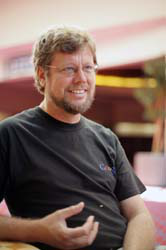
\includegraphics[width=3cm]{bdfl.png}
\end{figure}
\item Guido is also known as Benevolent Dictator For Life 
      (BDFL. See \url{http://tinyurl.com/5pg99q})
\end{itemize}
\end{frame}

% -----------------------------------------------
\begin{frame}[fragile]
\frametitle{Implementations (cont.)}
\begin{itemize}
\item There are other implementations as well.
\item IronPython (.NET CLR \url{http://ironpython.net})
\item Jython (Java VM \url{http://www.jython.org/})
\item pyjs (JavaScript \url{http://pyjs.org/})
\item Skulpt (web browser \url{http://www.skulpt.org})
\item CodeSkulptor (web browser \url{http://www.codeskulptor.org})
\end{itemize}
\end{frame}

% -----------------------------------------------
\begin{frame}[fragile]
\frametitle{Python 2 or 3?}
\begin{itemize}

\item Python 3.0 (2008) broke backward compatibility.
\begin{itemize}
\item Can't use 2 modules in 3 and vice versa.
\end{itemize}

\item "2 is legacy, 3 is the
       present and future." (\url{http://tinyurl.com/omgx9tk})
\begin{itemize}
\item 3.4 is expected in early 2014.
\item 2.0 was released in 2000.
\item 2.7 (2010) will be the last 2.x branch.
\end{itemize}

\item Many of 3's major futures have been backported to 2.6 and 2.7, 
      but not all. 
\item Other implementations in general still
      lack support for Python 3.
\end{itemize}
\end{frame}

% -----------------------------------------------
\begin{frame}[fragile]
\frametitle{Editors and IDE's}
\begin{itemize}
\item EMACS comes with python.el (24.2 and up) and
      python-mode.el (newer). See (\url{http://tinyurl.com/y67za8d})
\item VIM configuration links at \url{http://tinyurl.com/apx3avc}
\item IDLE (\url{http://tinyurl.com/c7j2k3x})
\item (Semi-) commercial editors, e.g., Komodo, PyCharm, Sublime, \ldots 
\item IPython (\url{http://ipython.org}) and IPython notebook.
\item And many others. See \url{http://tinyurl.com/leqyjw7}.
\end{itemize}
\end{frame}

% -----------------------------------------------
\begin{frame}[fragile]
\frametitle{IPython and IPython Notebook}
\begin{itemize}
\item A comprehensive environemnt for interactive and exploratory
      computing.
\item A ``new killer app'' back in 2011. 1.0 released in 2013.
\item One of the six core packages of SciPy stack.
\begin{figure}[h]
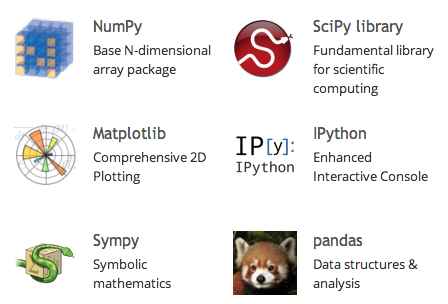
\includegraphics[width=8cm]{scipy.png}
\end{figure}
\end{itemize}
\end{frame}

% -----------------------------------------------
\begin{frame}[fragile]
\frametitle{PyPI and pip}
\begin{itemize}
\item Python Package Index (PyPI) is the repository 
      of software for Python at
      \url{http://pypi.python.org/pypi}.
\item As of a day in Jan 2014, it has about 38,800 packages.
\item Python Indexing Project (pip) (\url{http://www.pip-installer.org}) 
      is the standard tool for \emph{installing} packages
      (or modules) from PyPI. 
\item Some examples of using pip. At the shell prompt:
\begin{lstlisting}[language=bash,escapechar=\%]
$ pip
$ pip list
$ pip install SomePackage
$ pip install %\--\--%user SomePackage
$ pip install %\--\--%upgrade SomePackage
$ pip uninstall
\end{lstlisting}
\item Once a package is successfully installed,
      then you can \lstinline{import} the module
      within your script.
\end{itemize}
\end{frame}

% -----------------------------------------------
\begin{frame}[fragile]
\frametitle{Installing SciPy Stack}
\begin{itemize}
\item It \emph{is} possible to install all the packages
      one by one (and all the dependencies). It \emph{could}
      turn out to be tricky.
\item An alternative is to download and install free 
      or commercial distributions. Some names are:
      Anaconda, Enthought Canopy, Python(x,y), WinPython,
      \ldots
\item See \url{http://www.scipy.org/install.html}.
\item Check out Wakari.IO (\url{https://www.wakari.io})
      for playing with SciPy stack on the cloud, without
      local installation.
\end{itemize}
\end{frame}

% -----------------------------------------------
\begin{frame}[fragile]
\frametitle{Quiz}
\begin{itemize}
\item Choose the best one that fits each description:
\begin{enumerate}
\item Standard module supporting object (de-)serialization,
      which is written in C.
\item Compiler that turns Python source into efficient
      C code.
\item Software tool for installing / managing packages.
\item Benevolent Dictator For Life.
\item Provides a rich architecture for interactive (scientific) 
      computing. Version 1.0 was released in 2013.  
\end{enumerate}
\end{itemize}
\begin{tcolorbox}
          comprehension cPickle CPython Cython
          Guido van Rossum IPython Niklaus Wirth
          Pickle pip Sublime xrange()
          Yukihiro Matsumoto
\end{tcolorbox} 
\end{frame}

% -----------------------------------------------
\begin{frame}[fragile]
\frametitle{NumPy}
\begin{itemize}
\item Provides the \lstinline{ndarray} object.
\item \lstinline{ndarray} implements an efficient
      homogeneous multidimensional array.
\item Element-wise and vectorized matrix operations
      are provided.
\item Lots of modules use / built on NumPy.
\item Documentation at \url{http://docs.scipy.org/doc}.
\end{itemize}
\end{frame}

% -----------------------------------------------
\begin{frame}[fragile]
\frametitle{SciPy}
\begin{itemize}
\item Collection of mathematical algorithms and
      utility functions built on NumPy.
\item Organized into subpackages: cluster,
      constants, fftpack, integrate, interpolate, io, 
      linalg (linear algebra), ndimage (N-dimentional
      image processing), odr (orthogonal distance regression),
      optimize, signal (signal processing), 
      sparse (sparce matrices), spatial, special
      (functions), stats, weave (C/C++ integration)
\item Documentation at \url{http://docs.scipy.org/doc}.
\end{itemize}
\end{frame}

% -----------------------------------------------
\begin{frame}[fragile]
\frametitle{Matplotlib}
\begin{itemize}
\item Provides comprehensive 2D and simple 3D plotting.
\item Simple plot, Subplots (multiple axes),
      Histograms, Path, Simple 3D plot (surface, wireframe, scatter, bar),
      Streamlines (of a vector field), Ellipses,
      Bar charts, Pie charts, Filled (curves and polygons),
      Financial charts, Polar plots, \ldots, including TeX expressions support
      (internal or external) and Sketch plots (XKCD style)
\item Screenshots are (with source code) at 
      \url{http://matplotlib.org/users/screenshots.html}.
\item Documentation at \url{http://matplotlib.org/contents.html}.
\end{itemize}
\end{frame}

% -----------------------------------------------
\begin{frame}[fragile]
\frametitle{pandas}
\begin{itemize}
\item ``Python Data Analysis Library'' (Release 0.12 as of 2013).
\item \lstinline{Series}, \lstinline{DataFrame}
      , and \lstinline{Panel} objects
\item reading/writing data to and from: CSV,
      text file, Excel, SQL db, and fast HDF5 
      (scientific data file formats and libraries
       developed at NCSA), JSON, HTML Table, STATA.
\item Labeling columns, iteration, 
      Hierarchical Indexing, Transformation,
      Selection, Missing Data, Merge,
      Grouping (or split-apply-combine),
      Reshaping (or pivoting), Time Series,
      I/O tools, R interface (via rpy2).
\item Documentation at \url{http://pandas.pydata.org}.
\item Wes McKinney, ``10-minute tour of pandas''
      (\url{http://vimeo.com/59324550}) or workshop
      (\url{http://www.youtube.com/watch?v=MxRMXhjXZos})      
\end{itemize}
\end{frame}

% -----------------------------------------------
\begin{frame}[fragile]
\frametitle{Demonstration}
\begin{itemize}
\item Using IPython
\end{itemize}
\end{frame}

% -----------------------------------------------
\begin{frame}[fragile]
\frametitle{Learning Resources}
\begin{itemize}
\item Websites:
\begin{itemize}
\item Main website \url{http://www.python.org} and SciPy
      site \url{http://scipy.org}.
\item Official Python Tutorial
      \url{http://docs.python.org/2/tutorial/index.html}.
\item Google's Python Class (2 day class materials including
      video and exercises) 
      \url{https://developers.google.com/edu/python}.
\end{itemize}
\end{itemize}
\end{frame}

% -----------------------------------------------
\begin{frame}[fragile]
\frametitle{Learning Resources}
\begin{itemize}
\item Three advanced level tutorial videos:
\begin{itemize}
\item technical (old)
      \url{http://www.youtube.com/watch?v=E_kZDvwofHY}.
\item idioms (new) 
      \url{http://www.youtube.com/watch?v=OSGv2VnC0go}.
\item functional style
      \url{http://www.youtube.com/watch?v=Ta1bAMOMFOI}.
\item 2000+ videos at \url{http://pyvideo.org}.
\end{itemize}
\end{itemize}
\end{frame}

% -----------------------------------------------
\begin{frame}[fragile]
\frametitle{Learning Resources}
\begin{itemize}
\item Books:
\begin{itemize}
\item Mark Lutz (2013) \emph{Learning Python} 5th ed 
      (1,400 plus pages).
\item ``6 Free E-Books'' mentioned on 
      \url{http://tinyurl.com/m2y9rad}.
\item Matthew Russell (2013) ``Mining the Social Web''
      2nd edition is out. Example code files (in IPython
      Notebook file .ipynb format) are 
      at \url{http://tinyurl.com/n3txeu5}.
\end{itemize}
\end{itemize}
\end{frame}

% -----------------------------------------------
\begin{frame}[fragile]
\frametitle{Learning Resources}
\begin{itemize}
\item Any cool computer language has:
\begin{itemize}
\item Zen (read and memorize!)
      \url{http://www.python.org/dev/peps/pep-0020/}
\item Koans (unit testing)
      \url{http://tinyurl.com/7n6yfvn}
\item Challenges (old)
      \url{http://www.pythonchallenge.com/}
\end{itemize}
\item Need more challenges?
\begin{itemize}
\item Try the Project Euler
      \url{http://projecteuler.net}
\end{itemize}
\end{itemize}
\end{frame}

% -----------------------------------------------
\begin{frame}[fragile]
\frametitle{Learning Resources}
\begin{itemize}
\item MOOC's using Python extensively:
\begin{itemize}
\item ``Introduction to Computer Science and 
      Programming Using Python'' 
      (edX, \url{http://tinyurl.com/o3pbmc3})
\item ``Introduction to Interactive Programming in Python''
      (Coursera, \url{http://tinyurl.com/c95qh2q})
\item ``Coding the Matrix: Linear Algebra through Computer
      Science Applications'' (Coursera, 
      \url{http://tinyurl.com/awkbdho})
\end{itemize}
\end{itemize}
\end{frame}

% -----------------------------------------------
\begin{frame}[fragile]
\frametitle{Learning Resources}
\begin{itemize}
\item Twitter:
\begin{itemize}
\item "teaching python 140 character at a time": 
      \url{http://twitter.com/raymondh}
\end{itemize}
\item Gallery
\begin{itemize}
\item IPython Notebook gallery (including social data)
      \url{http://tinyurl.com/c5tj9xh}
\end{itemize}
\end{itemize}
\end{frame}

\end{document}
